\documentclass{article}
\usepackage{graphicx} % Required for inserting images
\usepackage{amsmath}
\usepackage{amssymb}   % Additional symbols, such as \mathbb and various math symbols
\usepackage{amsfonts}  % Additional fonts for mathematical symbols, like \mathbb
\usepackage{mathtools} % Extends amsmath with additional functionality
\usepackage{mathrsfs}  % Provides script fonts (\mathscr)
\usepackage{amsthm}    % Enhanced theorem environments (theorem, lemma, etc.)
\usepackage{bbm}
\usepackage{tikz}
\usetikzlibrary{shapes.geometric, calc}
\usepackage{array}
\usetikzlibrary{intersections, calc}
\usepackage{geometry}


\title{Applied Probability and Statistics I - STAT400}
\author{Tom Mitchell}
\date{Mestiyage - Fall 2024}

\begin{document}

\maketitle

\section*{Syllabus}

\subsection*{Grading}
\begin{itemize}
    \item Homework — 28\% (7\% each)
    \item R Projects — 12\% (4\% each)
    \item Two exams — 30\% (15\% each)
    \item Final exam — 30\%
\end{itemize}

\subsection*{Office Hours}
\begin{itemize}
    \item Tuesday: 1:00 PM - 1:50 PM (in person, MTH 4106)
    \item Wednesday: 11:00 AM - 11:50 AM (online)
\end{itemize}

\subsection*{Exams}
\begin{itemize}
    \item 2 midterms and a final exam
\end{itemize}

\section*{Lecture 1: Tuesday 8/27/2024}

\section*{Course Overview: STAT400}
We study:
\begin{enumerate}
    \item Probability
    \item Descriptive Statistics
    \item Inferential Statistics
\end{enumerate}

\pagebreak

\subsection*{1. Probability}
\textit{Probability} is the mathematical study of uncertainty.

\subsection*{2. Descriptive Statistics}
\textit{Descriptive Statistics} involves methods for summarizing and describing the important characteristics of a dataset.

\subsection*{3. Inferential Statistics}
\textit{Inferential Statistics} involves methods for using data from a subset (sample) of a larger group (population) to make meaningful conclusions. Note that each time you pick a subset, you lose out on certain information, leading to uncertainty.

\subsection*{Setting: Conducting an Experiment}

In this course, we will often assume we are about to conduct an experiment. The possible outcomes of the experiment are known, but the exact outcome is not.

\textbf{Examples:}
\begin{itemize}
    \item Tossing a coin
    \item Rolling a die
\end{itemize}

To study these types of situations, we introduce a \textit{model for probability}.

\subsection*{Ordered Triples (\(\Omega, \mathcal{F}, P\))}
\begin{itemize}
    \item \(\Omega\) is the \textbf{sample space}: The set of all possible outcomes of the experiment.
    \item \(\mathcal{F}\) is the \textbf{event space}:
    \begin{itemize}
        \item An \textbf{event} is a subset of \(\Omega\).
        \item An event captures the idea that in many situations, we care about collections of outcomes rather than a single outcome.
        \item The event space contains collections of outcomes for which we can assign probabilities.
    \end{itemize}
    \item \(P\) is the \textbf{probability measure}:
    \[
    P: \mathcal{F} \rightarrow \mathbb{R}
    \]
    where \(P\) assigns probabilities to events.

\end{itemize}

\pagebreak

\subsection*{Example 1: Tossing a Fair Coin}
Consider the simple experiment of tossing a \textbf{fair} coin.

\[
\Omega = \{H, T\}
\]

\[
\mathcal{F} = \{\emptyset, \{H\}, \{T\}, \{H, T\}\}
\]

\begin{itemize}
    \item \(P(\emptyset) = 0\) \\
    (``A probability of 0 represents an outcome/collection of outcomes that never takes place.")
    
    \item \(P(\{H, T\}) = 1\) \\
    (``A probability of 1 represents an outcome/collection of outcomes that always takes place.")
    
    \item \(P(\{H\}) = \frac{1}{2}\) \\
    (Requires the coin to be fair.)
    
    \item \(P(\{T\}) = \frac{1}{2}\) \\
    (Requires the coin to be fair.)
\end{itemize}

\subsection*{Example 2: Rolling a Fair Die}
Consider the experiment of rolling a fair die. Note: (\(\mathcal{P}(\Omega)\) is the Powerset of \(\Omega\))

\[
\Omega = \{1, 2, 3, 4, 5, 6\}
\]

\[
\mathcal{F} = \mathcal{P}(\Omega) =
\]
\[
\begin{aligned}
\{\emptyset, \{1\}, \{2\}, \ldots, \{6\}, \{1, 2\}, \ldots, \{1, 6\}, \{2, 3\}, \ldots, \\
\{1, 2, 3\}, \{2, 3, 4\}, \ldots, \{1, 2, 3, 4\}, \{1, 2, 3, 4, 5\}, \ldots, \Omega = \{1, 2, 3, 4, 5, 6\}\}
\end{aligned}
\]

\begin{itemize}
    \item \(P(\{i\}) = \frac{1}{6}\) for \(i = 1, 2, 3, 4, 5, 6\)
    \item \(P(\emptyset) = 0\)
    \item \(P(\Omega) = 1\)
    \item \(P(\{1, 2\}) = ?\) \\
    (Listing out probabilities for each event is \textbf{not} feasible.)
\end{itemize}

We would want a way to calculate the probability of a particular event by using the ``base" probabilities.

\textit{We will look at these rules for computing probabilities of complicated events in terms of basic ones in a bit.}

\subsection*{Example 3: Tossing a Fair Coin Until We See Heads for the First Time}
Consider the experiment of tossing a fair coin repeatedly until we observe heads for the first time, then we stop.

\[
\Omega = \{(H), (T, H), (T, T, H), (T, T, T, H), \ldots\}
\]

\[
\mathcal{F} = \mathcal{P}(\Omega)
\]

Let \(A_i\) be the event of seeing heads on the \(i\)th toss.

\[
P(A_i) = \frac{1}{2^i}
\]

\textbf{Question:} What is the probability of seeing heads on an even-numbered toss?

\[
Q = P(\text{seeing heads on an even-numbered toss}) = ?
\]

\subsection*{Example 4: Picking a Number from the Interval [0, 1]}
Consider picking a number from the interval \([0, 1]\) such that the probabilities of selecting numbers from two subintervals \(I_1\) and \(I_2\) of \([0, 1]\) are the same whenever \(I_1\) and \(I_2\) have the same length.

\[
\Omega = [0, 1]
\]

\[
\mathcal{F} = \mathcal{P}(\Omega)
\]

\[
P(\text{selecting a number from a subinterval } I \text{ of } [0, 1]) = \text{length}(I)
\]

\[
P([0, \frac{1}{4}]) = \frac{1}{4} - 0 = \frac{1}{4}
\]

\[
P([0, \frac{1}{2}]) = \frac{1}{2} - 0 = \frac{1}{2}
\]

\[
P\left(\left\{\frac{1}{2}\right\}\right) = P\left(\left[\frac{1}{2}, \frac{1}{2}\right]\right) = \frac{1}{2} - \frac{1}{2} = 0
\]

``The probability of 0 indicates an event that does not take place or an event that is so unlikely that the only reasonable value to assign to it is 0, i.e., an event that almost surely does not take place."

On Thursday will learn how to compute problems similar to \(P(\mathbb{Q} \cap [0, 1])\) = ?


\pagebreak

\section*{Lecture 2: Thursday 8/29/2024}

\subsection*{Probability}

\begin{itemize}
    \item Mathematical study of uncertainty.
\end{itemize}

\subsection*{Probability Space}

\[
(\Omega, F, P)
\]

\begin{itemize}
    \item \(\Omega\) - All possible outcomes of the experiment of interest.
    \item \(F\) - Contains events, i.e., collections of outcomes we would like to assign probabilities to.
    \item \(P\) - Probability measure.
\end{itemize}

\[
P: F \rightarrow \mathbb{R}
\]

On Tuesday, we discussed examples and introduced some formulas to compute probabilities of ``basic" events.

\subsection*{Goal for Today}

Explore how to compute probabilities of ``complicated" events in terms of basic events.

\subsection*{Two Questions}

\begin{enumerate}
    \item How do we express a complicated event in terms of basic ones?
    \item What rules can be used to compute probabilities once Question 1 has been answered?
\end{enumerate}

\begin{itemize}
    \item Question 1 is best answered by using tools from set theory.
\end{itemize}

\[
\rightarrow \text{We treat } \Omega \text{ as the list of all possible outcomes.}
\]
\[
\rightarrow \text{Events are sublists of } \Omega.
\]

Since we are only interested in outcomes (or combinations thereof) of the experiment, we treat \(\Omega\) as the universal set (i.e., we pretend that nothing outside of \(\Omega\) exists).

\subsection*{Pictorial Representation}

\begin{center}
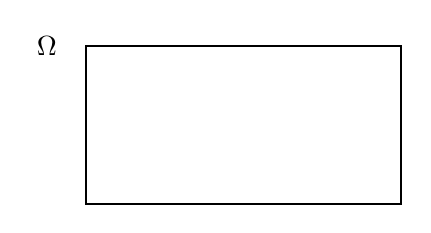
\begin{tikzpicture}
    \draw[thick] (0,0) rectangle (4,2);
    \node at (-0.5,2) {\(\Omega\)};
\end{tikzpicture}
\end{center}

\pagebreak

We can manipulate collections of events to obtain new events in various ways:

\begin{itemize}
    \item Intersections
    \item Unions
    \item Relative complements
\end{itemize}

Given events \(A\) and \(B\), the intersection is the event that contains all outcomes common to both \(A\) and \(B\). We denote this by \(A \cap B\).

\subsection*{Intersection of Two Events}

\begin{center}
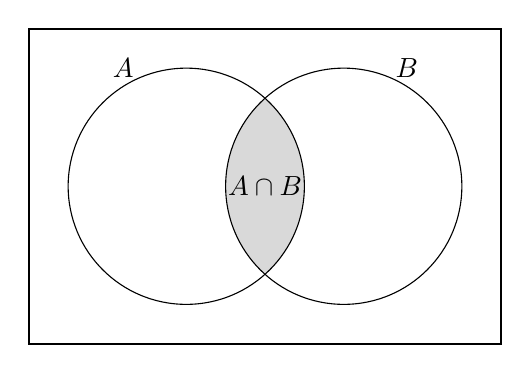
\begin{tikzpicture}
    % Draw the rectangle representing the universal set Omega
    \draw[thick] (-2,-2) rectangle (4,2);
    
    % Draw the circles representing sets A and B
    \begin{scope}
        \clip (0,0) circle(1.5);
        \fill[gray!30] (2,0) circle(1.5);
    \end{scope}
    \draw (0,0) circle(1.5);
    \draw (2,0) circle(1.5);
    
    % Label the sets
    \node at (-0.8,1.5) {\(A\)};
    \node at (2.8,1.5) {\(B\)};
    
    % Label the intersection area
    \node at (1,0) {\(A \cap B\)};
    
\end{tikzpicture}
\end{center}

\subsection*{Example}

\[
\Omega = \{1, 2, 3, 4, 5, 6\}
\]

Let \(A = \{1, 3, 5\}\) and \(B = \{4, 5\}\). Then, the intersection of \(A\) and \(B\) is:

\[
A \cap B = \{5\}
\]

\subsection*{Extending the Intersection to Families of Events}

The idea of the intersection of events can be extended to families of events.

\[
\bigcap_{i=1}^{3} A_i = (A_1 \cap A_2) \cap A_3
\]

For an infinite family of events:

\[
\bigcap_{i=1}^{\infty} A_i = A_1 \cap A_2 \cap A_3 \cap A_4 \cap A_5 \cap \ldots
\]


\subsection*{Disjoint Events}

Two events are said to be disjoint if \(A \cap B = \emptyset\).

\begin{itemize}
    \item Events \(A_1, \ldots, A_n\) are said to be disjoint if \(\textstyle \bigcap_{i=1}^{n} A_i = \emptyset \).

    \item Events \(A_1, \ldots, A_n, \ldots\) are said to be disjoint if \(\textstyle \bigcap_{i=1}^{\infty} A_i = \emptyset \).
 
    \item Events \(A_1, A_2, \ldots\) are said to be pairwise disjoint if \(A_i \cap A_j = \emptyset\) for all \(i \neq j\).
\end{itemize}

\subsection*{Example}

Consider the sample space \(\Omega = \{1, 2, 3, 4, 5, 6\}\) with the following events:

\[
A = \{1, 3, 5\}, \quad B = \{4, 5\}, \quad C = \{6\}
\]

Here, \(A\), \(B\), and \(C\) are disjoint events, meaning:

\[
A \cap B \cap C = \emptyset
\]

However, they are not pairwise disjoint, because:

\[
A \cap B = \{5\} \neq \emptyset
\]

\subsection*{Pairwise Disjoint Sets}

\begin{center}
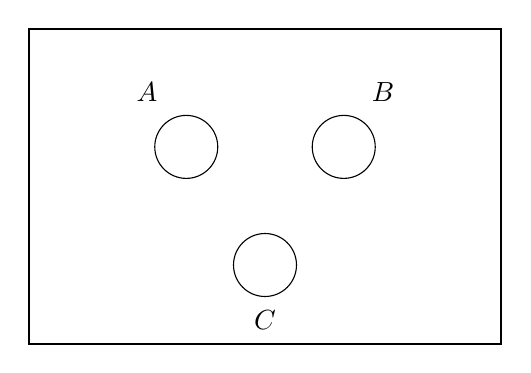
\begin{tikzpicture}

    % Draw the rectangle representing the universal set Omega
    \draw[thick] (-2,-2) rectangle (4,2);
    
    % Draw non-intersecting circles representing pairwise disjoint sets
    \draw (0,0.5) circle(0.4);
    \draw (2,0.5) circle(0.4);
    \draw (1,-1) circle(0.4);
    
    % Label the sets
    \node at (-0.5,1.2) {\(A\)};
    \node at (2.5,1.2) {\(B\)};
    \node at (1,-1.7) {\(C\)};
    
\end{tikzpicture}
\end{center}


The word ``and" usually translates to intersection when discussing sets or events. Conversely, the word ``or" translates to a union.

\subsection*{Unions}

The union of two events \(A\) and \(B\), denoted by \(A \cup B\), is the event that contains all outcomes that are in \(A\), \(B\), or both.

\subsection*{Venn Diagram: Union of Two Sets}

\begin{center}
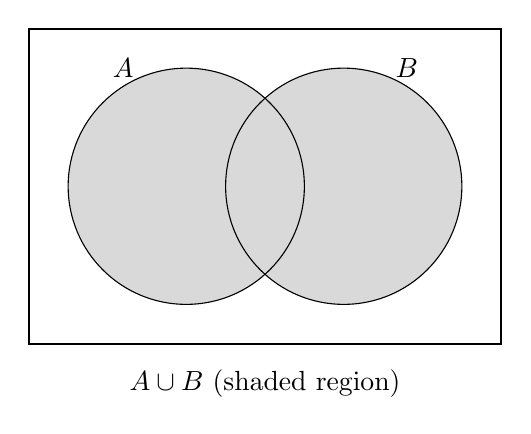
\begin{tikzpicture}

    % Draw the rectangle representing the universal set Omega
    \draw[thick] (-2,-2) rectangle (4,2);
    
    % Draw the circles representing sets A and B
    \begin{scope}
        \clip (0,0) circle(1.5);
        \fill[gray!30] (2,0) circle(1.5);
    \end{scope}
    \fill[gray!30] (0,0) circle(1.5);
    \fill[gray!30] (2,0) circle(1.5);
    \draw (0,0) circle(1.5);
    \draw (2,0) circle(1.5);
    
    % Label the sets
    \node at (-0.8,1.5) {\(A\)};
    \node at (2.8,1.5) {\(B\)};
    \node at (1,-2.5) {\(A \cup B\) (shaded region)};
    
\end{tikzpicture}
\end{center}

\subsection*{Example}

Consider the sample space \(\Omega = \{1, 2, 3, 4, 5, 6\}\) with the following events:

\[
A = \{1, 3, 5\}, \quad B = \{2, 3, 5\}
\]

The union of \(A\) and \(B\) is:

\[
A \cup B = \{1, 2, 3, 5\}
\]


\subsection*{Infinite and Finite Unions}

Infinite versions of unions and finite versions of unions with more than two sets can be similarly defined.

\[
\bigcup_{i=1}^{3} A_i = A_1 \cup A_2 \cup A_3
\]

Similarly, the union of more than two finite sets can be defined as:

\[
\bigcup_{i=1}^{n} A_i = A_1 \cup A_2 \cup \ldots \cup A_n
\]

Unions can also be extended to infinite collections of sets. For example, the union of an infinite sequence of sets \(A_1, A_2, \ldots\) is denoted as:

\[
\bigcup_{i=1}^{\infty} A_i = A_1 \cup A_2 \cup \ldots
\]



\subsection*{Relative Complements}

Given events \(A\) and \(B\), the relative complement \(A - B\) is the event that contains only the outcomes that are \textbf{unique} to \(A\).

\subsection*{Venn Diagram: Unique to A (\(A - B\))}

\begin{center}
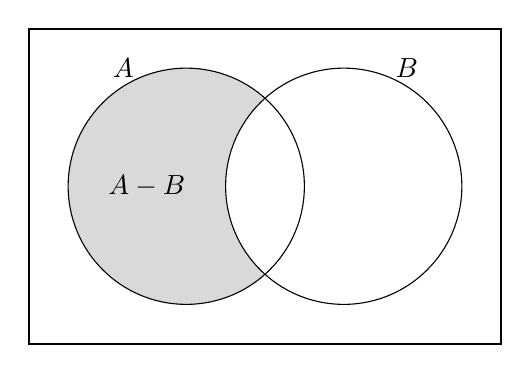
\begin{tikzpicture}

    % Draw the rectangle representing the universal set Omega
    \draw[thick] (-2,-2) rectangle (4,2);
    
    % Draw the circles representing sets A and B
    \fill[gray!30] (0,0) circle(1.5);
    \begin{scope}
        \clip (2,0) circle(1.5);
        \fill[white] (0,0) circle(1.5);
    \end{scope}
    \draw (0,0) circle(1.5);
    \draw (2,0) circle(1.5);
    
    % Label the sets
    \node at (-0.8,1.5) {\(A\)};
    \node at (2.8,1.5) {\(B\)};
    \node at (-0.5,0) {\(A - B\)};
    
\end{tikzpicture}
\end{center}

\subsection*{Example}

Consider the sample space \(\Omega = \{1, 2, 3, 4, 5, 6\}\) with the following events:

\[
A = \{1, 2, 3\}, \quad B = \{2, 4, 5\}
\]

The relative complements are:

\[
A - B = \{1, 3\}, \quad B - A = \{4, 5\}
\]


\subsection*{Complement of A}

We use \(A^c\) to denote the complement of \(A\) within the universal set \(\Omega\), which is the set of outcomes that are not in \(A\):

\[
A^c = \Omega - A = \{4, 5, 6\}
\]

The word \textbf{not} is associated with complements and the phrases ``and not", ``but not" are associated with relative compliments

\subsection*{Aside (for the HW): Verifying Set Identities with Venn Diagrams}

We can use Venn diagrams to verify set identities. For example, let's verify the identity:

\[
(A \cap B)^c = A^c \cup B^c
\]

Venn diagrams representing set operations of (left hand side) LHS and (right hand side) RHS respectively are shown below:

\begin{figure}[htbp]
\centering
\begin{tikzpicture}
    \node at (0, 3) {\textbf{LHS}};
    \node at (7, 3) {\textbf{RHS}};
    % Left Column - Top (A \cap B)
    \node at (0, 0) {
        \begin{tikzpicture}
            \node at (1,2.5) {\(A \cap B\)};
            % Draw the rectangle representing the universal set Omega
            \draw[thick] (-2,-2) rectangle (4,2);
            
            % Draw A and B with intersection filled
            \begin{scope}
                \clip (0,0) circle(1.5);
            \end{scope}
            \begin{scope}
                \clip (2,0) circle(1.5);
                \fill[gray!30] (0,0) circle(1.5);
            \end{scope}
            \draw (0,0) circle(1.5);
            \draw (2,0) circle(1.5);
            
            % Label the sets
            \node at (-0.8,1.5) {\(A\)};
            \node at (2.8,1.5) {\(B\)};
        \end{tikzpicture}
    };

    % Left Column - Bottom (Complement of A \cap B)
    \node at (0, -6) {
        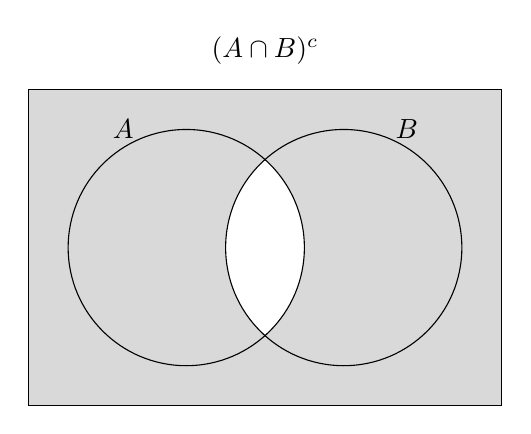
\begin{tikzpicture}
            \node at (1,2.5) {\((A \cap B)^c\)};
            % Draw the rectangle representing the universal set Omega
            \draw[thick] (-2,-2) rectangle (4,2);
            
            % Draw (A \cap B)^c
            \fill[gray!30] (-2,-2) rectangle (4,2);
            \begin{scope}
                \clip (0,0) circle(1.5);
            \end{scope}
            \begin{scope}
                \clip (2,0) circle(1.5);
                \fill[white!30] (0,0) circle(1.5);
            \end{scope}
            \draw (0,0) circle(1.5);
            \draw (2,0) circle(1.5);
            
            % Label the sets
            \node at (-0.8,1.5) {\(A\)};
            \node at (2.8,1.5) {\(B\)};
        \end{tikzpicture}
    };

    % Right Column - Top (A^c)
    \node at (7, 0) {
        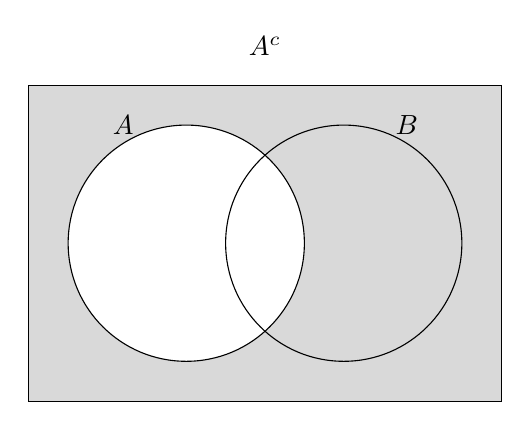
\begin{tikzpicture}
            \node at (1,2.5) {\(A^c\)};
            % Draw the rectangle representing the universal set Omega
            \draw[thick] (-2,-2) rectangle (4,2);
            
            % Draw complement of A
            \fill[gray!30] (-2,-2) rectangle (4,2);
            \fill[white] (0,0) circle(1.5);
            \draw (0,0) circle(1.5);
            \draw (2,0) circle(1.5);
            
            % Label the sets
            \node at (-0.8,1.5) {\(A\)};
            \node at (2.8,1.5) {\(B\)};
        \end{tikzpicture}
    };

    % Right Column - Middle (B^c)
    \node at (7, -6) {
        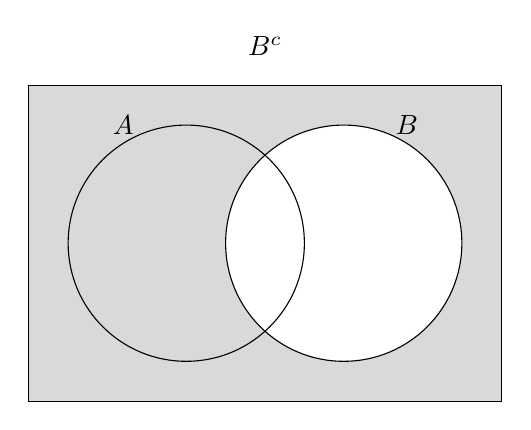
\begin{tikzpicture}
            \node at (1,2.5) {\(B^c\)};
            % Draw the rectangle representing the universal set Omega
            \draw[thick] (-2,-2) rectangle (4,2);
            
            % Draw complement of B
            \fill[gray!30] (-2,-2) rectangle (4,2);
            \fill[white] (2,0) circle(1.5);
            \draw (0,0) circle(1.5);
            \draw (2,0) circle(1.5);
            
            % Label the sets
            \node at (-0.8,1.5) {\(A\)};
            \node at (2.8,1.5) {\(B\)};
        \end{tikzpicture}
    };

    % Right Column - Bottom (A^c \cup B^c)
    \node at (7, -12) {
        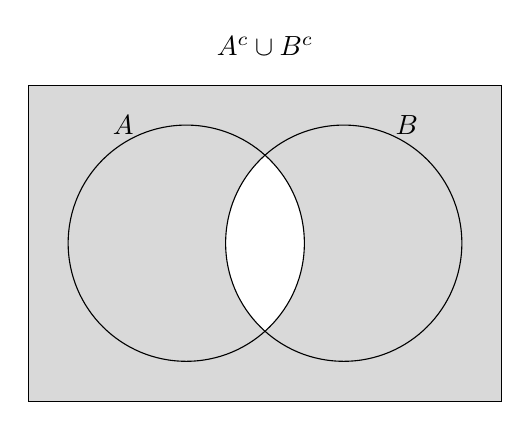
\begin{tikzpicture}
            \node at (1,2.5) {\(A^c \cup B^c\)};
            % Draw the rectangle representing the universal set Omega
            \draw[thick] (-2,-2) rectangle (4,2);
            
            % Draw A^c union B^c
            \fill[gray!30] (-2,-2) rectangle (4,2);
            \begin{scope}
                \clip (0,0) circle(1.5);
            \end{scope}
            \begin{scope}
                \clip (2,0) circle(1.5);
                \fill[white!30] (0,0) circle(1.5);
            \end{scope}
            \draw (0,0) circle(1.5);
            \draw (2,0) circle(1.5);
            
            % Label the sets
            \node at (-0.8,1.5) {\(A\)};
            \node at (2.8,1.5) {\(B\)};
        \end{tikzpicture}
    };

\end{tikzpicture}
\label{fig:venn-diagrams}
\end{figure}


\pagebreak

\subsubsection*{Conclusion}

Both sides of the identity are visually represented by the same shaded region, thus confirming that:

\[
(A \cap B)^c = A^c \cup B^c
\]


The shaded regions for \((A \cap B)^c\) and \(A^c \cup B^c\) match. Therefore, \((A \cap B)^c = A^c \cup B^c\). 

\[\]

\textbf{Note}: (we are not worrying about edges cases, for example, where A and B are disjoint but the identity still holds true)

\[\]
Now that the terminology is in place, we start to answer Q2.

\section*{Axioms}

\begin{enumerate}
    \item \(P(\Omega) = 1\), \(P(\emptyset) = 0\)
    \item \(P(A) \geq 0 \quad \text{for all } A \in \mathcal{F}\)
    \item If \(A_1, A_2, \ldots, A_n, \ldots \in \mathcal{F}\) are pairwise disjoint, then 
    \[
    P\left(\bigcup_{i=1}^{\infty} A_i\right) = \sum_{i=1}^{\infty} P(A_i)
    \]
\end{enumerate}


\textbf{Example:}
Consider the problem of tossing a fair coin until we observe heads. We want to find P(heads on an even numbered toss)

Let \( A \) be the event that heads appears for the first time on an even-numbered toss.

Thus, \( A \) can be expressed as:
\[
A = \{ (T, H), (T, T, T, H), (T, T, T, T, T, H), \dots \}
\]

Recall, $A_i$ is heads on the ith toss.


\[
P(A_i) = \frac{1}{2^i}
\]


Notice that we can describe \( A \) as the union of disjoint events where heads occurs for the first time on the \( 2i \)-th toss:

\[
A = A_2 \cup A_4 \cup A_6 \cup \dots = \bigcup_{i=1}^{\infty} A_{2i}
\]

where \( A_{2i} \) is the event that heads first appears on the \( 2i \)-th toss. The probability of \( A_{2i} \) can be computed as:
\[
P(A_{2i}) = \left(\frac{1}{2}\right)^{2i}
\]

Since the events \( A_{2i} \) are pairwise disjoint, we can use axiom 3 to see the probability of \( A \) is given by:
\[
P(A) = P\left(\bigcup_{i=1}^{\infty} A_{2i}\right)
= \sum_{i=1}^{\infty} P(A_{2i}) 
= \sum_{i=1}^{\infty} \left(\frac{1}{2}\right)^{2i} = \sum_{i=1}^{\infty} \left(\frac{1}{4}\right)^{i}
\]
This series is an infinite geometric series with the first term \( a = \frac{1}{4} \) and common ratio \( r = \frac{1}{4} \): 

Recall, that a the sum of a converging infinite geometric series where \(|r| < 1\) is:
\[
S = a+ar+ar^2+... = \sum_{i=0}^{\infty} \left(ar^n\right) = \frac{a}{1 - r}
\]

Therefore:
\[
\sum_{i=1}^{\infty} \left(\frac{1}{4}\right)^i = \frac{\frac{1}{4}}{1 - \frac{1}{4}} = \frac{\frac{1}{4}}{\frac{3}{4}} = \frac{1}{3}
\]

Thus, the probability that the first occurrence of heads is on an even-numbered toss is \( \boxed{\frac{1}{3}} \).


Derived rule: If \( A_1, \dots, A_N \in \mathcal{F} \) are pairwise disjoint, then 
\[
P\left(\bigcup_{i=1}^{\infty} A_i\right) = \sum_{i=1}^{\infty} P(A_i)
\]

\textbf{Example}: Consider a fair die roll. What is the probability of rolling a 1, 3, or 5?

\[
P(\{i\}) = \frac{1}{6} \quad \text{for } i = 1, \dots, 6
\]

\[
P(\{1, 3, 5\}) = P(\{1\}) + P(\{3\}) + P(\{5\}) = \frac{1}{6} + \frac{1}{6} + \frac{1}{6} = \frac{1}{2}
\]


\section*{Lecture 3: Thursday 9/3/2024}
\section{Probability}

\textbf{Definition:} Probability is the mathematical framework for quantifying and analyzing uncertainty.

A probability space is defined by the triple \( (\Omega, \mathcal{F}, P) \), where:
\begin{itemize}
    \item \( \Omega \) is the sample space (set of all possible outcomes)
    \item \( \mathcal{F} \) is the event space (sigma-algebra of subsets of \( \Omega \))
    \item \( P \) is the probability measure (function assigning probabilities to events)
\end{itemize}

\subsection*{Axioms of Probability}

The probability measure \( P \) satisfies the following axioms:
\begin{enumerate}
    \item \( P(\Omega) = 1 \) and \( P(\emptyset) = 0 \)
    \item For all \( A \in \mathcal{F} \), \( P(A) \geq 0 \)
    \item (Countable additivity) If \(A_1, A_2, \ldots \in \mathcal{F}\) are pairwise disjoint events (i.e $A_i \cap A_j = \emptyset$ for all $i \neq j$):
        \[
        P\left(\bigcup_{i=1}^{\infty} A_i\right) = \sum_{i=1}^{\infty} P(A_i)
        \]
\end{enumerate}

\textbf{Note:} Understanding and being able to derive properties from these axioms is crucial for the first midterm and for building a solid foundation in probability theory.

\subsection*{Important Results}

\begin{enumerate}  
    \item \textbf{Decomposition of Probability:} For any two events \(A, B \in \mathcal{F}\):
    \[
        P(B) = P(B - A) + P(A \cap B)
    \]

    \textit{Proof:} 
    \begin{itemize}
        \item Observe that \(B\) can be partitioned into two disjoint sets: \(B = (B - A) \cup (A \cap B)\)
        \item Note that \((B - A) \cap (A \cap B) = \emptyset\) (these sets are mutually exclusive)
        \item By the axiom of countable additivity (which implies finite additivity for disjoint events):
        \[P(B) = P((B - A) \cup (A \cap B)) = P(B - A) + P(A \cap B)\]
    \end{itemize}

    This result is fundamental in probability theory and is often used in solving complex probability problems. 
    It allows us to break down the probability of an event into mutually exclusive parts, which can be easier to calculate individually.

    \begin{center}
    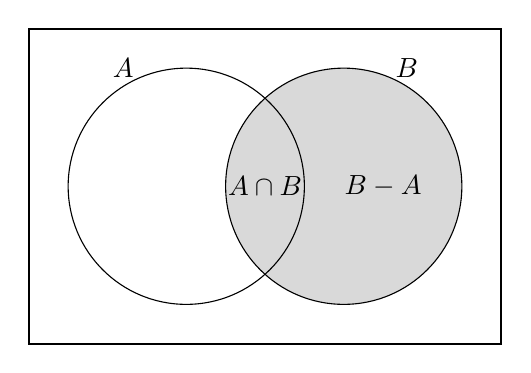
\begin{tikzpicture}
        % Draw the rectangle representing the universal set Omega
        \draw[thick] (-2,-2) rectangle (4,2);
        
        % Draw the circles representing sets A and B
        \fill[gray!30] (2,0) circle(1.5);
        \begin{scope}
            \clip (0,0) circle(1.5);
        \end{scope}
        \draw (0,0) circle(1.5);
        \draw (2,0) circle(1.5);
        
        % Label the sets
        \node at (-0.8,1.5) {\(A\)};
        \node at (2.8,1.5) {\(B\)};
        \node at (1,0) {\(A \cap B\)};
        \node at (2.5,0) {\(B - A\)};
    \end{tikzpicture}
    \end{center}
    \pagebreak
    \item \textbf{Finite Additivity:} For any two events \(A, B \in \mathcal{F}\):
    \[
        P(A \cup B) = P(A) + P(B) - P(A \cap B)
    \]

    \textit{Proof:}
    \begin{itemize}
        \item Observe that \(A \cup B = A \cup (B - A)\) and \(A \cap (B - A) = \emptyset\)
        \item Since \(A\) and \(B - A\) are disjoint, \(P(A \cup B) = P(A) + P(B - A)\) (finite additivity)
        \item From the decomposition result: \(P(B) = P(B - A) + P(A \cap B)\)
        \item Rearranging: \(P(B - A) = P(B) - P(A \cap B)\)
        \item Substituting into our earlier equation:
              \[P(A \cup B) = P(A) + P(B) - P(A \cap B)\]
    \end{itemize}
    
    \begin{center}
    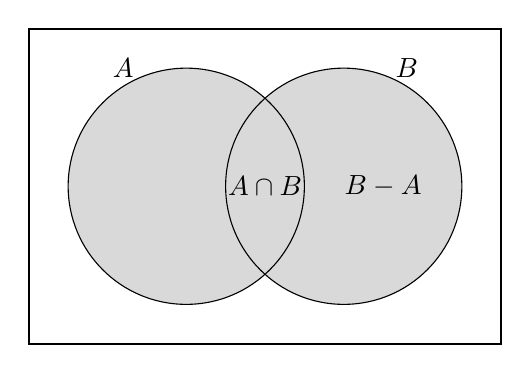
\begin{tikzpicture}
        % Draw the rectangle representing the universal set Omega
        \draw[thick] (-2,-2) rectangle (4,2);
        
        % Draw the circles representing sets A and B
        \fill[gray!30] (0,0) circle(1.5);
        \fill[gray!30] (2,0) circle(1.5);
        \draw (0,0) circle(1.5);
        \draw (2,0) circle(1.5);
        
        % Label the sets
        \node at (-0.8,1.5) {\(A\)};
        \node at (2.8,1.5) {\(B\)};
        \node at (1,0) {\(A \cap B\)};
        \node at (2.5,0) {\(B - A\)};
    \end{tikzpicture}
    \end{center}
    
    \item \textbf{Monotonicity:} If \(A \subseteq B\), then \(P(A) \leq P(B)\)
    
    \textit{Proof:} 
    \begin{itemize}
        \item If \(A \subseteq B\), then:
            \begin{itemize}
                \item \(B = A \cup (B - A)\)
                \item \(A \cap (B - A) = \emptyset\)
            \end{itemize}
        \item By finite additivity: \(P(B) = P(A \cup (B - A)) = P(A) + P(B - A)\)
        \item Since probabilities are non-negative, \(P(B - A) \geq 0\)
        \item Therefore, \(P(B) \geq P(A)\)
    \end{itemize}
    
    \begin{center}
    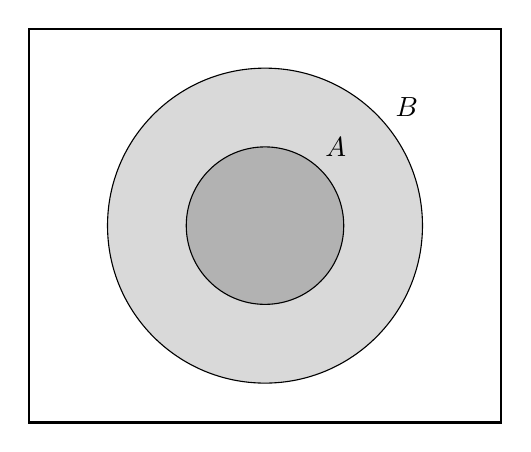
\begin{tikzpicture}
        % Draw the rectangle representing the universal set Omega
        \draw[thick] (-2,-2.5) rectangle (4,2.5);
        
        % Draw the circles representing sets A and B
        \fill[gray!30] (1,0) circle(2);
        \fill[gray!60] (1,0) circle(1);
        \draw (1,0) circle(2);
        \draw (1,0) circle(1);
        
        % Label the sets
        \node at (1.9,1) {\(A\)};
        \node at (2.8,1.5) {\(B\)};
    \end{tikzpicture}
    \end{center}
    
    \item \textbf{Union of Three Sets:} For \(A, B, C \in \mathcal{F}\):
    \[
    P(A \cup B \cup C)
    \]

    \textit{How to compute:}
    \begin{align*}
        P(A \cup B \cup C) &= P(A) + P(B \cup C) - P(A \cap (B \cup C)) \\
        &= P(A) + [P(B) + P(C) - P(B \cap C)] - P(A \cap (B \cup C)) \quad \text{(decompose the union)} \\
        &= P(A) + P(B) + P(C) - P(B \cap C) - P((A \cap B) \cup (A \cap C)) \quad \text{(by distributive law)} \\
        &= P(A) + P(B) + P(C) - P(B \cap C) - (P(A \cap B) + P(A \cap C) - P((A \cap B) \cap (A \cap C)))  \\
        &= P(A) + P(B) + P(C) - P(B \cap C) - (P(A \cap B) + P(A \cap C) - P(A \cap B \cap C))  \\
        &= P(A) + P(B) + P(C) - P(B \cap C) - P(A \cap B) - P(A \cap C) + P(A \cap B \cap C)  \\
    \end{align*}


\begin{center}
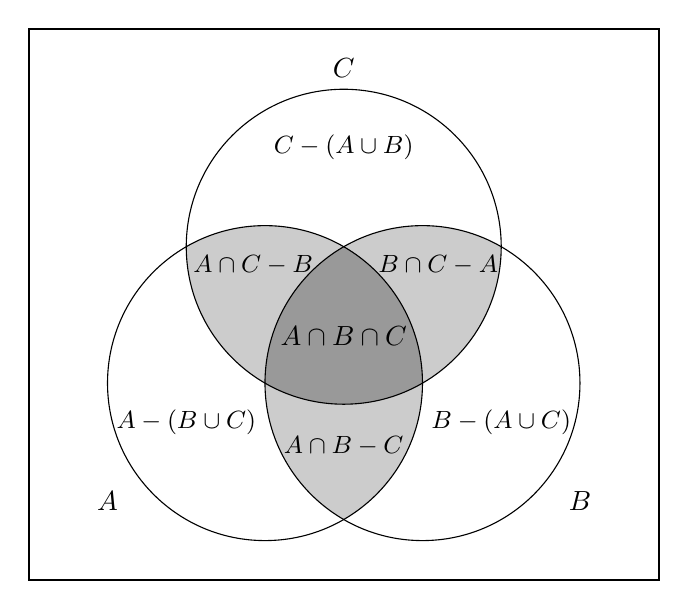
\begin{tikzpicture}
    % Draw the rectangle representing the universal set Omega
    \draw[thick] (-3,-2.5) rectangle (5,4.5);
    
    % Draw the circles representing sets A, B, and C
    \begin{scope}
        \clip (0,0) circle(2);
        \fill[gray!40] (2,0) circle(2);
        \fill[gray!40] (1,1.732) circle(2);
    \end{scope}
    \begin{scope}
        \clip (2,0) circle(2);
        \fill[gray!40] (1,1.732) circle(2);
    \end{scope}
    
    % Fill the intersection of all three circles with a darker shade
    \begin{scope}
        \clip (0,0) circle(2);
        \clip (2,0) circle(2);
        \fill[gray!80] (1,1.732) circle(2);
    \end{scope}
    
    \draw (0,0) circle(2);
    \draw (2,0) circle(2);
    \draw (1,1.732) circle(2);
    
    % Label the sets
    \node at (-2,-1.5) {\(A\)};
    \node at (4,-1.5) {\(B\)};
    \node at (1,4) {\(C\)};
    
    % Label intersections
    \node at (1,-0.8) {\small \(A \cap B - C\)};
    \node at (-0.15,1.5) {\small \(A \cap C - B\)};
    \node at (2.2,1.5) {\small \(B \cap C - A\)};
    \node at (1,0.6) {\(A \cap B \cap C\)};

    % Label regions for A, B, C only
    \node at (-1,-0.5) {\small $A - (B \cup C)$};
    \node at (3,-0.5) {\small $B - (A \cup C)$};
    \node at (1,3) {\small $C - (A \cup B)$};
    
    
\end{tikzpicture}
\end{center}


\end{enumerate}

\textbf{Example:} Suppose that $A$ and $B$ are events with $P(A) = 0.5$ and $P(B) = 0.6$. Find numbers $a$ and $b$ such that $a \leq P(A \cup B) \leq b$ and $a \leq P(A \cap B) \leq b$.

\begin{enumerate}
    \item Using the addition rule of probability:
        \[P(A \cup B) = P(A) + P(B) - P(A \cap B) = 0.5 + 0.6 - P(A \cap B) = 1.1 - P(A \cap B)\]
    
    \item Since $A \cup B \subseteq \Omega$ and $P(\Omega) = 1$, we have:
        \[P(A \cup B) \leq P(\Omega) \leq 1\]
    
    \item From steps 1 and 2:
        \[1.1 - P(A \cap B) \leq 1 \implies P(A \cap B) \geq 0.1\]
    
    \item The maximum value for $P(A \cap B)$ is $\min(P(A), P(B)) = 0.5$, because:
        \begin{itemize}
            \item $A \cap B \subseteq A$ and $A \cap B \subseteq B$
            \item Therefore, $P(A \cap B) \leq P(A)$ and $P(A \cap B) \leq P(B)$
        \end{itemize}
    
    \item We can conclude:
        \[0.1 \leq P(A \cap B) \leq 0.5\]
        \[0.6 \leq P(A \cup B) \leq 1.0\]
    
    \item To verify the lower bound for $P(A \cup B)$:
        \begin{align*}
            P(A \cup B) &= P(A) + P(B) - P(A \cap B) \\
                        &\geq P(A) + P(B) - \min(P(A), P(B)) \\
                        &= 0.5 + 0.6 - 0.5 = 0.6
        \end{align*}
\end{enumerate}

\textbf{Conclusion:} We have found that $a = 0.1$ and $b = 0.5$ satisfy $a \leq P(A \cap B) \leq b$, while $a = 0.6$ and $b = 1.0$ satisfy $a \leq P(A \cup B) \leq b$.

\textbf{Visualization:} To better understand the relationship between $A$ and $B$, consider the following Venn diagram:
\begin{center}
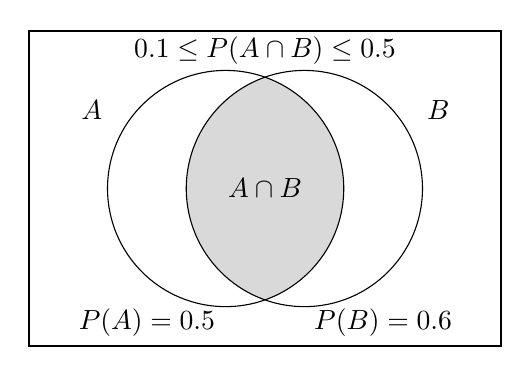
\begin{tikzpicture}
    % Draw the rectangle representing the universal set Omega
    \draw[thick] (-3,-2) rectangle (3,2);
    
    % Draw the circles representing sets A and B
    \begin{scope}
        \clip (-0.5,0) circle(1.5);
        \fill[gray!30] (0.5,0) circle(1.5);
    \end{scope}
    \draw (-0.5,0) circle(1.5);
    \draw (0.5,0) circle(1.5);
    
    % Label the sets
    \node at (-2.2,1) {$A$};
    \node at (2.2,1) {$B$};
    \node at (0, 0) {$A \cap B$};
    
    % Add probabilities
    \node at (-1.5,-1.7) {$P(A) = 0.5$};
    \node at (1.5,-1.7) {$P(B) = 0.6$};
    \node at (0,1.75) {$0.1 \leq P(A \cap B) \leq 0.5$};
\end{tikzpicture}
\end{center}

This visualization illustrates why $0.1 \leq P(A \cap B) \leq 0.5$ and $0.6 \leq P(A \cup B) \leq 1.0$.



\textbf{Example:} When Alice visits a certain grocery store, she:
\begin{itemize}
    \item buys apples with probability 0.4
    \item buys bananas with probability 0.7
    \item buys both with probability 0.25
\end{itemize}

Compute the probability that on her next visit to the store, Alice:
\begin{enumerate}
    \item buys either apples or bananas
    \item buys bananas but not apples
    \item buys neither apples nor bananas
\end{enumerate}

\textbf{Step 1:} Define notation and given probabilities
\begin{align*}
    A &: \text{Alice buys apples} \\
    B &: \text{Alice buys bananas}
\end{align*}

\begin{align*}
    P(A) &= 0.4 \\
    P(B) &= 0.7 \\
    P(A \cap B) &= 0.25
\end{align*}

\textbf{Note:} Symbol correspondences
\begin{itemize}
    \item $\cup$ corresponds to ``or" (union)
    \item $\cap$ corresponds to ``and" (intersection)
    \item $\complement$ corresponds to ``not" (complement)
    \item $-$ corresponds to ``and not", or ``but not" (relative complement)
\end{itemize}

\textbf{Step 2:} Calculate probabilities
\begin{enumerate}
    \item $P(A \cup B) = P(A) + P(B) - P(A \cap B) = 0.4 + 0.7 - 0.25 = 0.85$
    \item $P(B - A) = P(B) - P(A \cap B) = 0.7 - 0.25 = 0.45$
    \item $P(A^c \cap B^c) = P((A \cup B)^c) = 1 - P(A \cup B) = 1 - 0.85 = 0.15$
    
\end{enumerate}

\textbf{Note:} Important probability relationships:
\begin{align*}
    P(A) &= 1 - P(A^c) \\
    \Omega &= A \cup A^c \\
    P(\Omega) &= P(A) + P(A^c) = 1 \\
    P(A^c) &= 1 - P(A)
\end{align*}

\textbf{Computing probabilities for finite, equally likely outcomes:}
For any event $A \subseteq \Omega$, where $\Omega$ is a finite sample space with equally likely outcomes, the probability of $A$ is given by:

\[
P(A) = \frac{\text{number of elements in } A}{\text{number of elements in } \Omega} = \frac{|A|}{|\Omega|}
\]

where $|A|$ denotes the cardinality (number of elements) of set $A$.

\pagebreak

\section*{Lecture 4: Thursday 9/5/2024}

\subsection*{Probability for Finite, Equally Likely Outcomes}

Consider an experiment with finitely many outcomes, each of which is equally likely. This scenario is often referred to as ``fair" or ``uniformly at random" (with finite outcomes).

In this situation:
\begin{itemize}
    \item $\mathcal{F} = \mathcal{P}(\Omega)$
    \item For any event $A \in \mathcal{F}$, $P(A) = \frac{|A|}{|\Omega|}$
\end{itemize}

\textbf{Proof that $P(A) = \frac{|A|}{|\Omega|}$ satisfies the axioms of probability:}

\begin{enumerate}
    \item For any outcome $\omega \in \Omega$, we show $P(\{\omega\}) = \frac{1}{|\Omega|}$
    
    Let $\Omega = \{\omega_1, \omega_2, \ldots, \omega_n\}$. Then:
    \begin{itemize}
        \item $P(\{\omega_1\}) = P(\{\omega_2\}) = \cdots = P(\{\omega_n\})$ (equally likely)
        \item $\{\omega_i\}$ are pairwise disjoint for $i = 1, \ldots, n$
        \item $\Omega = \bigcup_{i=1}^{n} \{\omega_i\}$
        \item $P(\Omega) = P(\bigcup_{i=1}^{n} \{\omega_i\}) = \sum_{i=1}^{n} P(\{\omega_i\})$ (finite additivity)
    \end{itemize}
    Let $x = P(\{\omega_i\})$ for any $i$. Then:
    \begin{align*}
        1 &= P(\Omega) = nx \\
        x &= \frac{1}{n} = \frac{1}{|\Omega|}
    \end{align*}
    Therefore, $P(\{\omega_1\}) = P(\{\omega_2\}) = \cdots = P(\{\omega_n\}) = \frac{1}{|\Omega|}$

    \item For any event $A \subseteq \Omega$, we prove $P(A) = \frac{|A|}{|\Omega|}$
    
    Let $A = \{\omega_{i_1}, \omega_{i_2}, \ldots, \omega_{i_k}\}$ where $k = |A|$. Then:
    \begin{align*}
        P(A) &= P(\{\omega_{i_1}\} \cup \{\omega_{i_2}\} \cup \cdots \cup \{\omega_{i_k}\}) \\
             &= \sum_{j=1}^{k} P(\{\omega_{i_j}\}) \quad \text{(finite additivity)} \\
             &= \sum_{j=1}^{k} \frac{1}{n} \\
             &= \frac{k}{n} = \frac{|A|}{|\Omega|}
    \end{align*}
\end{enumerate}


To properly use the probability formula, we need to be able to count effectively. There are two fundamental principles of counting:

\begin{itemize}
    \item Additive principle of counting
    \item Multiplicative principle of counting
\end{itemize}

\textbf{Additive Principle of Counting:} If we have $n$ ways of doing one thing and $m$ ways of doing another thing, where both actions cannot be performed simultaneously, then there are $n + m$ ways of selecting an action.

\textbf{Example (Additive Principle):}
Suppose you own:
\begin{itemize}
    \item 6 pairs of jeans
    \item 5 pairs of slacks
\end{itemize}
Then there are $6 + 5 = 11$ ways of selecting an article of clothing.

\textbf{Multiplicative Principle of Counting:} If we have $n$ ways of doing one thing and $m$ ways of doing another thing, then there are $n \times m$ ways of performing both actions.

\textbf{Example (Multiplicative Principle):}
Continuing from the previous example, if you are packing for a trip and want to pack:
\begin{itemize}
    \item 1 pair of jeans
    \item 1 pair of slacks
\end{itemize}
There are $6 \times 5 = 30$ ways of selecting a pair of jeans and a pair of slacks.

Problems we study in this class can be categorized according to two main features:

\begin{enumerate}
    \item Replacement
    \item Order
\end{enumerate}

\noindent
Examples:
\begin{itemize}
    \item Passwords: Replacement allowed, order matters
    \item Card games: Usually no replacement, order may or may not matter (depends on the situation)
\end{itemize}

\noindent
We can visualize these categories in a 2x2 grid:

\begin{center}
\begin{tabular}{|c|c|c|}
    \hline
    & \textbf{Replacement} & \textbf{No Replacement} \\
    \hline
    \textbf{Order Matters} & \checkmark & \checkmark \\
    \hline
    \textbf{Order Doesn't Matter} & $\times$ & \checkmark \\
    \hline
\end{tabular}
\end{center}

\noindent
This grid helps us classify different probability problems based on their characteristics.
The $\checkmark$ and $\times$ are used to indicate what we will study in this class.


\textbf{Problem:} Suppose that a password consists of 10 characters. The character set contains 256 possible characters. If characters are chosen uniformly at random, what is the probability of picking a password that starts with an `A'?

\textbf{Analysis:}
\begin{itemize}
    \item Replacement: \checkmark
    \item Order matters: \checkmark
\end{itemize}

\textbf{Visualization:}
\begin{itemize}
    \item All possible passwords: 
        \[256, 256, 256, \ldots, 256\]
        \[\_\,\_\,\_\,\_\,\_\,\_\,\_\,\_\,\_\,\_\]
        (256 choices for each of the 10 slots)
    \item Passwords starting with 'A':
        \[A, 256, 256, \ldots, 256\]
        \[A\,\_\,\_\,\_\,\_\,\_\,\_\,\_\,\_\,\_\]
        (1 choice for first slot (`A'), 256 choices for each of the remaining 9 slots)
\end{itemize}

\textbf{Calculation:}
\begin{itemize}
    \item Total number of possible passwords: $256^{10}$ (256 choices for each of 10 slots)
    \item Number of passwords starting with `A': $1 \times 256^9$ (1 choice for first slot, 256 choices for each of 9 slots)
    \item Probability = $\frac{\text{Favorable outcomes}}{\text{Total outcomes}} = \frac{1 \times 256^9}{256^{10}} = \frac{1}{256}$
\end{itemize}

\textbf{Conclusion:} The probability of picking a password that starts with an `A' is $\frac{1}{256}$.

\noindent
\textbf{General Rule:} If you have a list of $n$ things to choose from, replacement is allowed, order matters, and you choose $k$ times, then there are $n^k$ possible choices.

\vspace{0.5cm}

\noindent
\textbf{New Problem:} Using the previous example (where $n = 256$ and $k = 10$), what is the probability of randomly picking a password that repeats at least one character?

\vspace{0.3cm}

\noindent
\textbf{Strategy:} It is sometimes easier to calculate the probability of the complement of an event.

\vspace{0.3cm}

\noindent
\textbf{Approach:} We will count the number of passwords where each character is unique.

\vspace{0.3cm}

\noindent
Let $A$ be the event that the randomly chosen password has no repeated characters.

$P(A^c) = 1 - P(A)$


\textbf{Number of passwords with unique characters:}
\begin{itemize}
    \item Visualization:
        \[\underbrace{256 \cdot 255 \cdot 254 \cdot 253 \cdot 252 \cdot 251 \cdot 250 \cdot 249 \cdot 248 \cdot 247}_{10\text{ positions}}\]
    \item Mathematical representation: $\prod_{i=0}^{9} (256 - i)$
    \item Probability calculation: $P(A^c) = 1 - \frac{\prod_{i=0}^{9} (256 - i)}{256^{10}}$
\end{itemize}

\vspace{0.5cm}

\pagebreak
\noindent
\textbf{General Formula:} When picking $k$ things out of $n$ things while keeping track of the order (where $k \leq n$):

\vspace{0.3cm}

\noindent
Number of different ways:
\begin{align*}
    &= n \cdot (n-1) \cdot (n-2) \cdot \ldots \cdot (n-k+1) \\
    &= n \cdot (n-1) \cdot (n-2) \cdot \ldots \cdot (n-k+1) \cdot \frac{(n-k) \cdot (n-k-1) \cdot \ldots \cdot 1}{(n-k) \cdot (n-k-1) \cdot \ldots \cdot 1} \\
    &= \frac{n!}{(n-k)!}
\end{align*}

Where $n!$ is defined as:
\[
    n! = \prod_{i=1}^{n} i \quad \text{and} \quad 0! = 1
\]

\vspace{0.3cm}

\noindent
$\frac{n!}{(n-k)!}$ is known as ``$n$ permute $k$", denoted as ${}^nP_k$.

\vspace{0.5cm}

\noindent
\textbf{No replacement, order does not matter:}

\noindent
The trick is to solve the problem assuming order matters, then adjust by dividing by the number of ways to order the $k$ things.

\vspace{0.3cm}

\noindent
Consider the following slots:

\[
\underbrace{\_\,\_\,\_\,\_\,\_\,\_\,\_\,\_\,\_\,\_}_{k\text{ slots}}
\]

\noindent
First, we count the number of ways to fill these slots while keeping track of the order:
\begin{itemize}
    \item This is given by ${}^nP_k = \frac{n!}{(n-k)!}$
    \item It represents the number of ways to choose and arrange $k$ items from $n$ options
\end{itemize}

However, this count includes permutations of the same $k$ items, which we don't want to distinguish. To adjust for this overcounting:
\begin{itemize}
    \item We divide by the number of ways to order $k$ items, which is $k!$
        \begin{itemize}
            \item $k!$ represents all possible permutations of the $k$ chosen items
        \end{itemize}
    \item This adjustment gives us the following formula:
        \[ \frac{{}^nP_k}{k!} = \frac{n!}{k!(n-k)!} = {}^nC_k = \binom{n}{k} \]
\end{itemize}

The result, $\binom{n}{k}$, is known as ``$n$ choose $k$". It represents the number of ways to choose $k$ items from $n$ options when the order doesn't matter.

\pagebreak

\section*{Lecture 5: Tuesday 9/10/2024}

\subsection*{No Replacement, Order Does Not Matter}

A common source of examples for this scenario is card games like poker.

\vspace{0.3cm}

\noindent
\textbf{Example:} Suppose you are dealt 5 cards from a well-shuffled deck of cards. What is the probability that you are dealt a straight (5 cards in sequence)?

\begin{itemize}
    \item A well-shuffled deck means all 52 cards are equally likely to be drawn (uniformly at random).
    \item A straight has 5 consecutive ranks but not all of the same suit.
\end{itemize}

\vspace{0.3cm}

\noindent
\textbf{Common Strategy: Undercount and Adjust}
\begin{itemize}
    \item We count a specific case and adjust for the number of cases.
    \item Recall: For $\binom{n}{k} = \frac{{}^nP_k}{k!}$, we overcounted and adjusted by dividing by $k!$.
\end{itemize}

\vspace{0.3cm}

\noindent
Let's consider a specific type of straight: one containing the ranks 9, 10, J, Q, K.

\begin{itemize}
    \item There are 4 different suits, so there are four ways to choose each rank.
    \item Total number of ways for a specific straight: $4^5 = 1024$
    \item Subtract straight flushes: $1024 - 4 = 1020$ (4 straight flushes, one for each suit)
\end{itemize}

The number of all straights is equal to $(4^5-4) \times$ number of options for the starting rank.

\begin{itemize}
    \item Ace can be considered the highest or lowest rank, but not both:
    \begin{itemize}
        \item A, 2, 3, 4, 5 \checkmark
        \item 10, J, Q, K, A \checkmark
        \item J, Q, K, A, 2 $\times$
    \end{itemize}
    \item There are 10 possible starting ranks (Ace(1) through 10)
\end{itemize}

    Therefore, the total number of straights is:

    \[ 10 \times (4^5-4) = 10 \times 1020 = 10,200 \]

    The required probability is:
    
    \begin{align*}
    P(\text{Straight}) &= \frac{\text{Number of straights}}{\text{Number of possible hands}} \\[6pt]
    &= \frac{10(4^5-4)}{\binom{52}{5}}
    \end{align*}

    \subsection*{Conditional Probability}

    Conditional probability measures the likelihood of an event occurring given that another event has already occurred. It allows us to update our probability estimates based on new information.
    
    \textbf{Definition:} Given two events $A$ and $B$, where $P(A) > 0$, the conditional probability of $B$ given that $A$ has occurred is denoted by $P(B|A)$. This probability is defined as:
    
    \[
    P(B|A) = \frac{P(A \cap B)}{P(A)}
    \]
    
    \textbf{Example:} Suppose you buy a lottery ticket and the first four numbers drawn match the numbers on your ticket. Your chances of winning have increased because we now have additional information.
    
    The formula for conditional probability can be interpreted as the proportion of outcomes in A that also belong to B. This is visually represented in the Venn diagram below:
    \begin{center}
    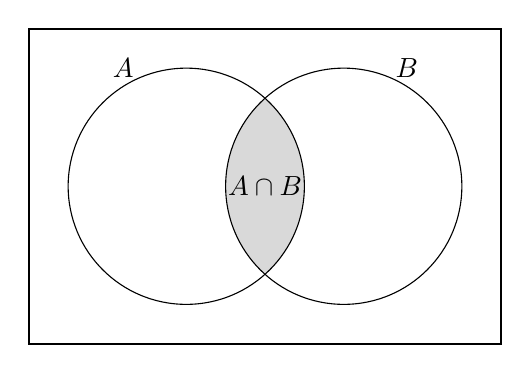
\begin{tikzpicture}
        % Draw the rectangle representing the universal set Omega
        \draw[thick] (-2,-2) rectangle (4,2);
        
        % Draw the circles representing sets A and B
        \begin{scope}
            \clip (0,0) circle(1.5);
            \fill[gray!30] (2,0) circle(1.5);
        \end{scope}
        \draw (0,0) circle(1.5);
        \draw (2,0) circle(1.5);
        
        % Label the sets
        \node at (-0.8,1.5) {$A$};
        \node at (2.8,1.5) {$B$};
        
        % Label the intersection area
        \node at (1,0) {$A \cap B$};
        
    \end{tikzpicture}
    \end{center}
    In this diagram, $P(B|A)$ represents the proportion of the area of $A$ that overlaps with $B$.
    
    \subsection*{Independence}
    
    Two events $A$ and $B$ are independent if:
    
    \[
    P(A \cap B) = P(A) \cdot P(B)
    \]

    \textbf{Note:} This definition holds for all values of $P(A)$ and $P(B)$, including when either or both equal zero.
    
    In the case where $P(A) > 0$, independence implies:
    
    \[
    \frac{P(A \cap B)}{P(A)} = P(B)
    \]
    
    Which is equivalent to $P(B|A) = P(B)$, meaning the occurrence of $A$ does not affect the probability of $B$.
    
    
    \section*{Lecture 6: Tuesday 9/12/2024}
    
    \subsection*{Review: Conditional Probability and Independence}
    
    On Tuesday, we discussed conditional probability and independence.
    
    \begin{itemize}
        \item Conditional Probability: $P(B|A) = \frac{P(A \cap B)}{P(A)}$, where $P(A) > 0$
        \item We added the requirement $P(B) > 0$, not necessary for the equation to hold true, but useful for computing $P(A|B)$ based on $P(B|A)$
    \end{itemize}
    
    \subsection*{Independence}
    
    Events $A$ and $B$ are independent if $P(A \cap B) = P(A)P(B)$
    
    If we assume $P(A) > 0$, then $P(B) = \frac{P(A \cap B)}{P(A)} = P(B|A)$
    
    \subsection*{Example: Rolling Two Fair Dice}
    
    Consider an experiment of rolling two fair dice. Alice and Bob are given the following question:
    
    \begin{quote}
    If Alice rolls the dice and tells Bob that the sum of the dice was 4, does this give Bob new information about whether the number 2 was rolled on the first die?
    \end{quote}
    
    \subsubsection*{Analysis}
    
    \begin{itemize}
        \item Sample Space: $\Omega = \{(i,j) | i,j = 1,2,3,4,5,6\}$
        \item $P(\{i,j\}) = \frac{1}{6} \cdot \frac{1}{6} = \frac{1}{36}$ (assuming independence)
        \item Alternate approach: All outcomes are equally likely
    \end{itemize}
    
    Let's define events:
    \begin{itemize}
        \item $A$: The sum of the numbers is 4
        \item $B$: The first die roll results in a 2
    \end{itemize}
    
    \begin{align*}
        A &= \{(1,3), (2,2), (3,1)\} \\
        B &= \{(2,1), (2,2), (2,3), (2,4), (2,5), (2,6)\} \\
        A \cap B &= \{(2,2)\}
    \end{align*}
    
    \begin{align*}
        P(B) &= \frac{6}{36} = \frac{1}{6} \\
        P(A \cap B) &= \frac{1}{36} \\
        P(B|A) &= \frac{P(A \cap B)}{P(A)} = \frac{\frac{1}{36}}{\frac{3}{36}} = \frac{1}{3} \neq \frac{1}{6} = P(B)
    \end{align*}
    Therefore, Alice's information does give Bob new information about the probability of rolling a 2 on the first die.

    \subsection*{Independence as an Assumption}

    It's important to note that independence is often an assumption, and it may not always be justified. Consider the following example:

    \subsubsection*{Sally Clark Case and SIDS}

    In the Sally Clark case, a misuse of probability led to a wrongful conviction:

    \begin{itemize}
        \item Probability of SIDS (Sudden Infant Death Syndrome) was estimated as $\frac{1}{7000}$
        \item Probability of two SIDS deaths was calculated as $(\frac{1}{7000})^2 = \frac{1}{49 \times 10^6}$
        \item This low probability was incorrectly interpreted as indicating guilt
    \end{itemize}

    However, this calculation had two major flaws:
    \begin{enumerate}
        \item The assumption of independence was not justified
        \item Low probability events do occur
    \end{enumerate}

    \subsection*{Frequentist Interpretation of Probability}

    The frequentist interpretation of probability is defined as:

    \[
    P(A) = \lim_{n \to \infty} \frac{\text{number of times A occurred}}{n}
    \]

    where $n$ is the number of independent repetitions of the experiment.

    \subsubsection*{Example: Fair Coin Toss}

    For a fair coin toss:

    \[
    P(\text{H}) = \frac{1}{2} = \lim_{n \to \infty} \frac{\text{number of heads}}{n}
    \]

    In practice, we approximate this as:

    \[
    P(\text{H}) \approx \frac{\text{number of heads observed}}{\text{total number of tosses}}
    \]

    \textbf{Note:} R Project 2 includes exercises related to these concepts.

    \subsection*{Bayes' Theorem - Required Terminology \& Proving Intermediate Results}
    
    \textbf{Note:} This will be on the list of proofs for exams.
    
    \subsubsection*{Partition}
    
    A partition of $\Omega$ is a collection of sets $\{A_\alpha : \alpha \in A\}$ such that:
    
    \begin{enumerate}
        \item $A_\alpha \cap A_\beta = \emptyset$ for all $\alpha, \beta \in A$ and $\alpha \neq \beta$
        \item $\bigcup_{\alpha \in A} A_\alpha = \Omega$
    \end{enumerate}

    Here is a visual example of a partition:
    
    \begin{center}
    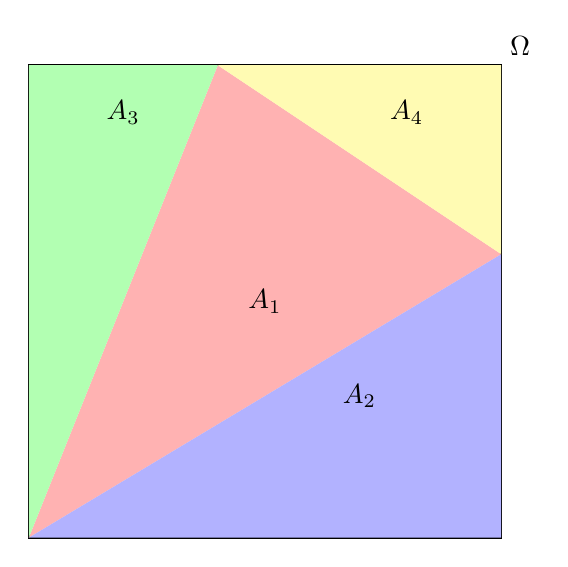
\begin{tikzpicture}[scale=1.2]
        % Sample space
        \draw[thick] (0,0) rectangle (5,5);
        \node at (5.2,5.2) {$\Omega$};
        
        % Partition elements
        \fill[red!30] (0,0) -- (2,5) -- (5,3) -- cycle;
        \fill[blue!30] (0,0) -- (5,0) -- (5,3) -- cycle;
        \fill[green!30] (0,0) -- (2,5) -- (0,5) -- cycle;
        \fill[yellow!30] (2,5) -- (5,3) -- (5,5) -- cycle;
        
        % Labels
        \node at (2.5,2.5) {$A_1$};
        \node at (3.5,1.5) {$A_2$};
        \node at (1,4.5) {$A_3$};
        \node at (4,4.5) {$A_4$};
    \end{tikzpicture}
    \end{center}
    
    A partition breaks up the sample space into distinct, non-overlapping pieces.

    Note:

    1) Given $A \subseteq \Omega$, the intersections $\{A \cap A_\alpha : \alpha \in \mathcal{A}\}$ form a partition of $A$.
    
    Here is a visual example:

    \begin{center}
    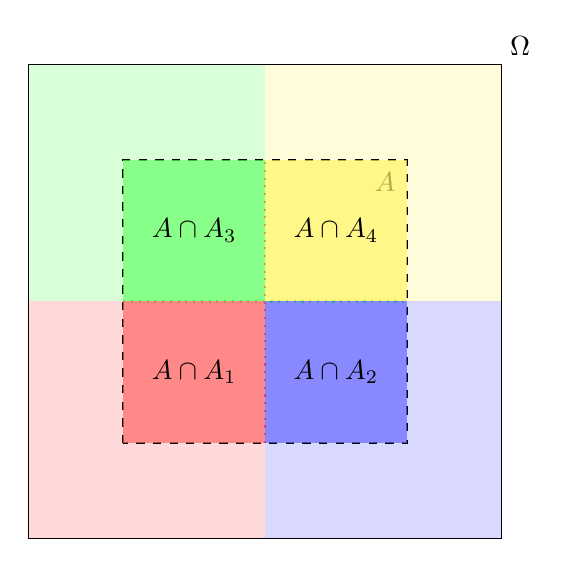
\begin{tikzpicture}[scale=1.2]
        % Draw the sample space
        \draw[thick] (0,0) rectangle (5,5);
        \node at (5.2,5.2) {$\Omega$};
        
        % Define partition lines
        \draw[dotted, thick, red] (2.5,0) -- (2.5,5) node[midway, right] {$A_2$};
        \draw[dotted, thick, green] (0,2.5) -- (5,2.5) node[midway, above] {$A_3$};
        
        % Fill partition regions with light colors
        \fill[red!15] (0,0) rectangle (2.5,5); % A1
        \fill[blue!15] (2.5,0) rectangle (5,2.5); % A2
        \fill[green!15] (0,2.5) rectangle (2.5,5); % A3
        \fill[yellow!15] (2.5,2.5) rectangle (5,5); % A4
        
        % Draw set A with thick dashed line
        \draw[thick, dashed] (1,1) rectangle (4,4) node[pos=0.85, above right] {$A$};
        
        % Draw dotted lines inside A to show partitions
        \draw[dotted, thick, red] (2.5,1) -- (2.5,4);
        \draw[dotted, thick, green] (1,2.5) -- (4,2.5);
        
        % Fill intersections within A with solid colors
        \fill[red!60, opacity=0.7] (1,1) rectangle (2.5,2.5); % A ∩ A1
        \fill[blue!60, opacity=0.7] (2.5,1) rectangle (4,2.5); % A ∩ A2
        \fill[yellow!60, opacity=0.7] (2.5,2.5) rectangle (4,4); % A ∩ A4
        \fill[green!60, opacity=0.7] (1,2.5) rectangle (2.5,4); % A ∩ A3
        
        % Labels for intersections
        \node at (1.75,1.75) {$A \cap A_1$};
        \node at (3.25,1.75) {$A \cap A_2$};
        \node at (3.25,3.25) {$A \cap A_4$};
        \node at (1.75,3.25) {$A \cap A_3$};
        
    \end{tikzpicture}
    \end{center}
    
    We typically consider problems where the partition $\{A_i\}$ is finite. That is, the partition splits up the sample space into finitely many non-overlapping pieces. For example, we might have $|\{A_i\}| = 2$ or $|\{A_i\}| = 3$.

    \vspace{0.5cm}

    \textbf{Law of Total Probability}

    Let $\{A_1, \ldots, A_n\}$ be a partition of the sample space $\Omega$ with $P(A_i) > 0$ for all $i$, and let $B$ be an event with $P(B) > 0$. Then:

    \begin{equation*}
    P(B) = \sum_{i=1}^n P(A_i \cap B) = \sum_{i=1}^n P(B|A_i)P(A_i)
    \end{equation*}

    This law allows us to calculate the probability of an event $B$ by considering its interaction with each part of the partition.


    \section*{Lecture 7: Tuesday 9/17/2024}

    \subsection*{Conditional Probability}

    \begin{itemize}
        \item \textbf{Definition of Conditional Probability}
        \item \textbf{Independence}
        \item \textbf{Bayes' Theorem}
    \end{itemize}

    \subsubsection*{Partition}
    A \textbf{partition} of the sample space \(\Omega\) is a collection \( \{B_1, \dots, B_n\} \) of events such that:
    \begin{align*}
        B_i \cap B_j &= \emptyset \quad \text{for all } i \neq j, \\
        \bigcup_{i=1}^{n} B_i &= \Omega.
    \end{align*}

    The diagrams above illustrate how the sample space is split into non-overlapping regions.

    \subsubsection*{Law of Total Probability}
    Suppose that \( \{B_1, \dots, B_n\} \) is a partition of the sample space \(\Omega\) with \( P(B_i) > 0 \) for all \(i\). Then, for any event \( A \) with \( P(A) > 0 \), we have:
    \[
        P(A) = \sum_{i=1}^{n} P(A \cap B_i) = \sum_{i=1}^{n} P(A \mid B_i) P(B_i)
    \]

    Consider the event \( A \), where 
    \[
        A = \bigcup_{i=1}^{n} (A \cap B_i)
    \]

    Note that the events \( A \cap B_i \) are pairwise disjoint (as shown in the above diagram).

    \[
        P(A) = P\left( \bigcup_{i=1}^{n} A \cap B_i \right) = \sum_{i=1}^{n} P(A \cap B_i)
    \]

    Additionally, the conditional probability is given by:
    \[
        P(A \mid B_i) = \frac{P(A \cap B_i)}{P(B_i)}
    \]

    Therefore:
    \[
        P(A \cap B_i) = P(A \mid B_i) P(B_i)
    \]
    \[
        P(A) = \sum_{i=1}^{n} P(A \mid B_i) P(B_i)
    \]

    \subsubsection*{Bayes' Theorem}
    
    Suppose \( B_1, B_2, \ldots, B_n \) is a partition of the sample space \( \Omega \) with \( P(B_i) > 0 \) for all \( i \). Let \( A \) be an event with \( P(A) > 0 \). Then, for any \( k \) where \( 1 \leq k \leq n \),
    
    \[
        P(B_k \mid A) = \frac{P(A \mid B_k) P(B_k)}{\sum_{j=1}^{n} P(A \mid B_j) P(B_j)}
    \]
    
    \textbf{Proof:} By the definition of conditional probability,
    
    \[
        P(B_k \mid A) = \frac{P(A \cap B_k)}{P(A)} = \frac{P(A \mid B_k) P(B_k)}{P(A)}
    \]
    
    Using the Law of Total Probability,
    
    \[
        P(A) = \sum_{j=1}^{n} P(A \mid B_j) P(B_j)
    \]
    
    Therefore,
    
    \[
        P(B_k \mid A) = \frac{P(A \mid B_k) P(B_k)}{\sum_{j=1}^{n} P(A \mid B_j) P(B_j)}
    \]
    
    The Law of Total Probability allows us to change the order of conditioning.
    
    \textbf{Example:} Suppose an experiment consists of tossing a fair coin followed by rolling a fair die if the coin comes up heads, and rolling a fair four-sided die if it comes up tails.
    
    What is the probability that we see heads given that we see a one?
    
    Let \( H \) be the event that the coin comes up heads, and \( F \) be the event that the die rolls a one. Then,
    
    \[
        P(F) = P(F \mid H) P(H) + P(F \mid T) P(T)
    \]
    
    \begin{figure}[h!]
        \centering
        \begin{tikzpicture}[
            grow=right,
            level distance=4cm,
            sibling distance=10cm,
            every node/.style={align=center, font=\small}
        ]
            \node {Start}
                child { 
                    node {Heads (H)}
                        edge from parent node[midway, above] {\(\frac{1}{2}\)}
                        child [sibling distance=1.5cm] {
                            child { node {1} edge from parent node[midway, above] {\(\frac{1}{6}\)} }
                            child { node {2} edge from parent node[midway, above] {\(\frac{1}{6}\)} }
                            child { node {3} edge from parent node[midway, above] {\(\frac{1}{6}\)} }
                            child { node {4} edge from parent node[midway, above] {\(\frac{1}{6}\)} }
                            child { node {5} edge from parent node[midway, above] {\(\frac{1}{6}\)} }
                            child { node {6} edge from parent node[midway, above] {\(\frac{1}{6}\)} }
                        }
                }
                child { 
                    node {Tails (T)}
                        edge from parent node[midway, below] {\(\frac{1}{2}\)}
                        child [sibling distance=1.5cm] {
                            child { node {1} edge from parent node[midway, above] {\(\frac{1}{4}\)} }
                            child { node {2} edge from parent node[midway, above] {\(\frac{1}{4}\)} }
                            child { node {3} edge from parent node[midway, above] {\(\frac{1}{4}\)} }
                            child { node {4} edge from parent node[midway, above] {\(\frac{1}{4}\)} }
                        }
                };
        \end{tikzpicture}
        \caption{Experiment Diagram: Coin Toss and Die Roll}
        \label{fig:coin-die-diagram}
    \end{figure}

    \textbf{Solution:}
    
    We are to find \( P(H \mid F) \).

    Using Bayes' Theorem,

    \[
        P(H \mid F) = \frac{P(F \mid H) \cdot P(H)}{P(F \mid H) \cdot P(H) + P(F \mid T) \cdot P(T)}
    \]

    Plugging in the values,

    \[
        P(H \mid F) = \frac{\left(\frac{1}{6}\right) \cdot \left(\frac{1}{2}\right)}{\left(\frac{1}{6} \cdot \frac{1}{2}\right) + \left(\frac{1}{4} \cdot \frac{1}{2}\right)} 
        = \frac{\frac{1}{12}}{\frac{1}{12} + \frac{1}{8}} 
        = \frac{\frac{1}{12}}{\frac{5}{24}} 
        = \frac{2}{5}
    \]

    Therefore, the probability that the coin was heads given that we saw a one is \( \boxed{\frac{2}{5}} \).

    \[
        \Omega = \{ (H, 1), (H, 2), (H, 3), (H, 4), (H, 5), (H, 6), (T, 1), (T, 2), (T, 3), (T, 4) \}
    \]

    \textbf{Bayes' Theorem:} Let \( H \) be the event that the coin comes up heads, and \( T \) be the event that it comes up tails.

    \begin{itemize}
        \item \( P(H) = \frac{1}{2} = P(T) \)
        \item \( H \cup T = \Omega \)
        \item \( H \cap T = \emptyset \)
    \end{itemize}

    Thus, \( H \) and \( T \) form a partition of \( \Omega \).

    \[
        P(i \mid H) = \frac{1}{6} \quad \text{for all } i \in \{1, 2, 3, 4, 5, 6\}
    \]

    \[
        P(i \mid T) = \frac{1}{4} \quad \text{for all } i \in \{1, 2, 3, 4\}
    \]

    \textbf{Bayes' Theorem:}
    
    \[
        P(\text{Heads} \mid \text{One}) = \frac{P(\text{One} \mid \text{Heads}) \cdot P(\text{Heads})}{P(\text{One} \mid \text{Heads}) \cdot P(\text{Heads}) + P(\text{One} \mid \text{Tails}) \cdot P(\text{Tails})}
    \]
    
    \bigskip
    
    \textbf{Problem Statement:}
    
    A doctor is called to see a sick child in a particular neighborhood (nhd). The doctor has prior information that sick children in the nhd are suffering from either measles or the flu, and no child has both. Additionally, the doctor knows that:
    \begin{itemize}
        \item \(90\%\) of sick children have measles.
        \item The probability that a child with measles has a rash is \(0.95\).
        \item The probability that a child with the flu has a rash is \(0.08\).
    \end{itemize}
    
    The child that the doctor sees has a rash. What is the probability that the child has measles?
    
    \bigskip
    
    \textbf{Definitions:}
    \begin{itemize}
        \item \(\Omega\): Sick children from the nhd.
        \item \(M\): The child has measles.
        \item \(F\): The child has the flu.
        \item \(R\): The child has a rash.
    \end{itemize}
    
    \(M\) and \(F\) form a partition of the sample space \(\Omega\).
    
    \bigskip
    
    \textbf{Given:}
    \[
        P(M) = 0.1, \quad P(F) = 0.9
    \]
    \[
        P(R \mid M) = 0.95, \quad P(R \mid F) = 0.08
    \]
    
    \bigskip
    
    \textbf{Applying Bayes' Theorem:}
    \[
        P(M \mid R) = \frac{P(R \mid M) \cdot P(M)}{P(R \mid M) \cdot P(M) + P(R \mid F) \cdot P(F)}
    \]
    
    \[
        = \frac{0.95 \times 0.1}{0.95 \times 0.1 + 0.08 \times 0.9}
    \]
    
    \[
        = \frac{0.095}{0.095 + 0.072} = \frac{0.095}{0.167} \approx 0.569
    \]
    
    \bigskip
    
    \textbf{Conclusion:} The probability that the child has measles given that the child has a rash is approximately \( \boxed{0.569} \).

    Suppose that you have 3 cards identical in every way except for their color. One card is red on both sides, one card is blue on both sides, and one card is red on one side and blue on the other. 
    You put the cards into a hat and mix them up. You pick one and put it on a desk. You see the color red. What is the probability that the other side is blue?

    \bigskip

    Let \(RR\) denote card 1, \(BB\) denote card 2, and \(RB\) denote card 3.

    Let \(R\) be the event that we see red when we put the card on the desk.

    \(RB\), \(BB\), and \(RR\) form a partition of \(\omega\).

    \[
        P(RB) = P(BB) = P(RR) = \frac{1}{3}
    \]

    \[
        P(R \mid RB) = \frac{1}{2}, \quad P(R \mid BB) = 0, \quad P(R \mid RR) = 1
    \]

    \[
        P(RB \mid R) = \frac{P(R \mid RB) \cdot P(RB)}{P(R \mid RR) \cdot P(RR) + P(R \mid RB) \cdot P(RB) + P(R \mid BB) \cdot P(BB)}
    \]

    \[
        P(RB \mid R) = \frac{\left(\frac{1}{2}\right) \cdot \left(\frac{1}{3}\right)}{\left(\frac{1}{2}\right) \cdot \left(\frac{1}{3}\right) + 0 \cdot \left(\frac{1}{3}\right) + 1 \cdot \left(\frac{1}{3}\right)} = \frac{\frac{1}{6}}{\frac{1}{6} + 0 + \frac{1}{3}} = \frac{\frac{1}{6}}{\frac{1}{2}} = \frac{1}{3}
    \]


    \section*{Lecture 8: Thursday 9/19/2024}

    \section*{Random Variables}

    A \textbf{random variable} is a function from the sample space to the real numbers.
    \[
        X : \Omega \to \mathbb{R}
    \]

    \textbf{Notes:}
    \begin{itemize}
        \item The actual definition has a lot more technicalities to rule out pathologies. We will not worry about these.
    \end{itemize}

    Random variables are based on the fact that in many situations we care about a value associated with our pick from the sample space rather than the pick itself.

    \textit{Example:} A study involving the effect of a new medication on blood pressure.

    A random variable is a function. Thinking in terms of examples may better highlight why the terminology is what it is.

    In order for a random variable to be useful, we should be able to compute 
    \[
        P(X \in A) = P(\{\omega : X(\omega) \in A\})
    \]
    for \(A \subseteq \mathbb{R}\).

    \(P(X \in A)\) is the probability of running across an outcome that causes the function to take a value inside of \(A\).

    \textit{Example (cont):}
    \[
        P(X \in [119, 125]) = P(\{\omega \mid X(\omega) \in [119, 125]\})
    \]

    \textbf{How do we convey this information?}

    \textbf{Distribution function for a random variable \(X\):}
    \[
        D_X : \mathcal{P}(\mathbb{R}) \to \mathbb{R}
    \]
    \[
        D_X(A) = P(X \in A)
    \]

    Since \(\mathcal{P}(\mathbb{R})\) contains very complicated subsets of real numbers, it is unlikely that we are able to express \(D_X\) in a form that is suitable for computation.

    For a random variable \(X\), the \textbf{cumulative distribution function} (CDF) is defined as:
    \[
        F_X : \mathbb{R} \to \mathbb{R}
    \]
    \[
        F_X(a) = P(X \leq a) = P(X \in (-\infty, a])
    \]

    Suppose that an experiment consists of tossing a fair coin. Let \(X\) track the outcome of the coin toss in the natural way. (\(\Omega = \{H, T\}\)) Define \(X(T) = 0\) and \(X(H) = 1\). Compute the CDF and the distribution function of \(X\).

    \[
        F_X(a) = P(X \leq a) = P(X \in (-\infty, a])
    \]

    Suppose \(a = -1.32975\):
    \[
        F_X(a) = P(X \leq a) = 0
    \]
    since no outcome of \(X\) can have a value less than \(a\).

    Note, this is true for any \(a < 0\):
    \[
        F_X(a) = 0 \quad \text{for all } a < 0
    \]

    \[
        F_X(0) = P(X \leq 0) = \frac{1}{2}
    \]

    Suppose \(a = 0.5\):
    \[
        F_X(a) = P(X \leq 0.5) = P(X = 0) = \frac{1}{2}
    \]

    Suppose \(a = 1\):
    \[
        F_X(a) = P(X \leq a) = P(X \leq 1) = P(X = 0 \text{ or } X = 1) = 1
    \]

    Suppose \(a > 1\):
    \[
        F_X(a) = P(X \leq a) = P(X \leq 1) = 1
    \]
    since any outcome of \(X\) must be less than or equal to 1.

    \[
        F_X(a) = 
        \begin{cases} 
            0 & \text{if } a < 0 \\
            0.5 & \text{if } 0 \leq a < 1 \\
            1 & \text{if } a \geq 1 
        \end{cases}
    \]

    \begin{enumerate}
        \item \(\lim_{a \to -\infty} F_X(a) = 0\)
        \item \(\lim_{a \to \infty} F_X(a) = 1\)
        \item \(F_X\) is monotonically increasing, i.e., if \(a < b\), \(F_X(a) \leq F_X(b)\)
        \item \(F_X\) is right continuous, i.e., \(\lim_{a \to a^+} F_X(a) = F_X(a)\)
    \end{enumerate}

    \textbf{Definition:} \(X\) and \(Y\) are said to have the same distribution if \(D_X(A) = D_Y(A)\) for all \(A \subseteq \mathbb{R}\). (i.e., \(X\) and \(Y\) cannot be distinguished by looking at the probabilities alone.)

    \textbf{Example:}

    Generate the numbers 0 and 1 so that both are equally likely.
    \begin{itemize}
        \item Toss a fair coin.
        \item Pick a number uniformly at random from the interval \([0, 1]\).
    \end{itemize}

    \(Y: [0, 1] \rightarrow \mathbb{R}\)
    \[
        Y(\omega) = 
        \begin{cases} 
            0 & \text{if } 0 < \omega < \frac{1}{2} \\
            1 & \text{if } \frac{1}{2} < \omega < 1 
        \end{cases}
    \]

    We cannot tell \(X\) and \(Y\) apart by looking at probabilities alone.

    \textbf{Fact:} \(D_X = D_Y\) if and only if \(F_X = F_Y\).

    \[
        D_X(A) = 
        \begin{cases} 
            0 & \text{if } 0, 1 \not\in A \\
            0.5 & \text{if } \{0\}, \{1\} \subseteq A \text{ but not } \{0, 1\} \subseteq A \\
            1 & \text{if } \{0, 1\} \subseteq A 
        \end{cases}
    \]

    \(D_X(A) = P(X \in A)\)

    \textbf{Example:} Suppose you roll a fair die.

    Let \(Y: \Omega \rightarrow \mathbb{R}\) be given by \(Y(\omega) = \omega\), where \(\Omega = \{1, 2, 3, 4, 5, 6\}\).

    What is \(F_Y\)?

    Case 1: \(a < 1\)
    \[
        F_Y(a) = 0
    \]

    Case 2: \(1 \leq a < 2\)
    \[
        F_Y(a) = P(Y \leq a) = P(\{1\}) = \frac{1}{6}
    \]

    Case 3: \(2 \leq a < 3\)
    \[
        F_Y(a) = P(Y \leq a) = P(\{1, 2\}) = \frac{2}{6} = \frac{1}{3}
    \]

    Case 4: \(3 \leq a < 4\)
    \[
        F_Y(a) = P(Y \leq a) = P(\{1, 2, 3\}) = \frac{3}{6} = \frac{1}{2}
    \]

    Case 5: \(4 \leq a < 5\)
    \[
        F_Y(a) = P(Y \leq a) = P(\{1, 2, 3, 4\}) = \frac{4}{6} = \frac{2}{3}
    \]

    Case 6: \(5 \leq a < 6\)
    \[
        F_Y(a) = P(Y \leq a) = P(\{1, 2, 3, 4, 5\}) = \frac{5}{6}
    \]

    Case 7: \(a \geq 6\)
    \[
        F_Y(a) = P(Y \leq a) = P(\{1, 2, 3, 4, 5, 6\}) = 1
    \]




























\end{document}
